\documentclass[11pt, aspectratio=169]{beamer}

% Gọi file cấu hình chung
\usepackage{./common_style}
\usepackage{tikz} % Thêm thư viện để vẽ hình
\usetikzlibrary{arrows.meta} % Thư viện để tùy chỉnh mũi tên

\title[VECTOR]{VECTOR}

% Thêm [Trần Đức Mạnh] để Beamer chỉ in tên ở chân trang các slide khác
% Còn trang bìa vẫn in toàn bộ khối tên + ngày + ảnh
\author[Trần Đức Mạnh]{
    Trần Đức Mạnh \\[0.2cm] 
    \today \\[0.4cm] 
    
\includegraphics[width=0.4\textwidth]{"/home/trandmanh/Projects/Funix/images/plane travel.png"}
} 


\titlegraphic{}

\begin{document}

% Trang tiêu đề
\begin{frame}
    \titlepage
\end{frame}

\section{Định nghĩa Vector}
\begin{frame}[fragile]{\insertsubsection}
    % Dùng lệnh này để đưa tên Section lên dòng 1 của tiêu đề slide
    \frametitle{\thesection. \insertsection}
    \vspace{-1cm}

    \begin{dinhnghia}
        Vector là một đoạn thẳng có hướng, nghĩa là đã chỉ rõ điểm đầu và điểm cuối.
    \end{dinhnghia}

    \begin{itemize}
        \item Kí hiệu: $\vec{AB}$, $\vec{a}$, $\vec{b}$.
        \item Độ dài của vector $\vec{AB}$ kí hiệu là $|\vec{AB}|$.
    \end{itemize}
    
    \begin{block}{Ghi chú}
        Vector có điểm đầu trùng điểm cuối gọi là vector không ($\vec{0}$).

        Với điểm A có tọa độ $(x_A, y_A)$ và điểm B có tọa độ $(x_B, y_B)$, vector $\vec{AB}$ có tọa độ là $(x_B - x_A, y_B - y_A)$.
    \end{block}
\end{frame}

\subsection{Vector trong mặt phẳng tọa độ Oxy (Vector in Coordinate Plane Oxy)}

% --- PHẦN HÌNH ẢNH MINH HỌA MỚI ---
\begin{frame}[fragile]{\insertsubsection}
        % Dùng lệnh này để đưa tên Section lên dòng 1 của tiêu đề slide
    \frametitle{\thesection. \insertsection}
    
    % Dùng lệnh này để đưa tên Subsection xuống dòng 2 (nhỏ hơn)
    \framesubtitle{\thesection.\thesubsection. \insertsubsection}
    % Đẩy toàn bộ nội dung lên một chút để tránh sát chân trang
    \vspace*{-0.2cm} 
    
    \begin{columns}[t] % Căn lề trên (top) để phần tiêu đề ảnh đều nhau
        % CỘT BÊN TRÁI
        \begin{column}{0.48\textwidth}
            \centering
            {\small \textbf{Vector $\vec{a}$ tại gốc $O$}} \\[0.1cm] % Giảm khoảng cách từ 0.5 xuống 0.1
            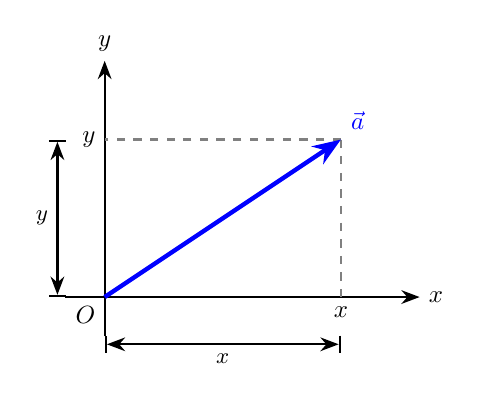
\begin{tikzpicture}[>=Stealth, thick, scale=1, every node/.style={scale=0.9}]
                % Hệ trục
                \draw[->] (-0.5,0) -- (4,0) node[right] {$x$};
                \draw[->] (0,-0.5) -- (0,3) node[above] {$y$};
                \node[below left] at (0,0) {$O$};

                % Đường gióng
                \draw[dashed, gray] (3,2) -- (3,0) node[below, black] {$x$};
                \draw[dashed, gray] (3,2) -- (0,2) node[left, black] {$y$};

                % Vector a
                \draw[->, blue, ultra thick] (0,0) -- (3,2) node[above right] {$\vec{a}$};

                % Ký hiệu độ dài x và y (Thêm y cho đủ bộ)
                \draw[|<->|] (0,-0.6) -- (3,-0.6) node[midway, below] {\small $x$};
                \draw[|<->|] (-0.6,0) -- (-0.6,2) node[midway, left] {\small $y$};
            \end{tikzpicture}
        \end{column}

        % CỘT BÊN PHẢI
        \begin{column}{0.48\textwidth}
            \centering
            {\small \textbf{Vector $\vec{AB}$ bất kỳ}} \\[0.1cm]
            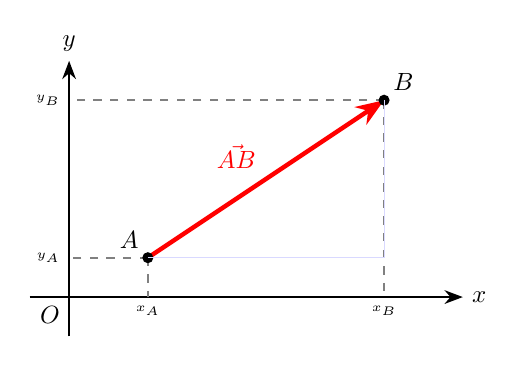
\begin{tikzpicture}[>=Stealth, thick, scale=1, every node/.style={scale=0.9}]
                % Hệ trục
                \draw[->] (-0.5,0) -- (5,0) node[right] {$x$};
                \draw[->] (0,-0.5) -- (0,3) node[above] {$y$};
                \node[below left] at (0,0) {$O$};

                % Tọa độ A và B
                \coordinate (A) at (1,0.5);
                \coordinate (B) at (4,2.5);
                
                \draw[dashed, gray] (A) -- (1,0) node[below, black] {\tiny $x_A$};
                \draw[dashed, gray] (A) -- (0,0.5) node[left, black] {\tiny $y_A$};
                \draw[dashed, gray] (B) -- (4,0) node[below, black] {\tiny $x_B$};
                \draw[dashed, gray] (B) -- (0,2.5) node[left, black] {\tiny $y_B$};

                % Vẽ vector AB
                \draw[->, red, ultra thick] (A) -- (B) node[midway, above left] {$\vec{AB}$};
                \fill (A) circle (2pt) node[above left] {$A$};
                \fill (B) circle (2pt) node[above right] {$B$};
                
                % Tam giác vuông mờ minh họa Pytagore
                \draw[blue!15, thin] (1,0.5) -- (4,0.5) -- (4,2.5);
            \end{tikzpicture}
        \end{column}
    \end{columns}

    % Điều chỉnh khoảng cách giữa hình và chữ
    \vspace{0.1cm}
    
    \begin{itemize}
        \item \footnotesize \textbf{Bên trái:} $\vec{a} = (x; y)$. Độ dài (Length)-cạnh huyền: $|\vec{a}| = \sqrt{x^2 + y^2}$.
        \item \footnotesize \textbf{Bên phải:} $\vec{AB} = (x_B - x_A; y_B - y_A)$. Độ dài (Length)-cạnh huyền : $|\vec{AB}| = \sqrt{(x_B - x_A)^2 + (y_B - y_A)^2}$.
    \end{itemize}
\end{frame}


\section{Các phép toán của vector (Vector Operations)}

\subsection{Phép công hai vector (Sum of vector)}

\begin{frame}[fragile]
    % Dùng lệnh này để đưa tên Section lên dòng 1 của tiêu đề slide
    \frametitle{\thesection. \insertsection}
    
    % Dùng lệnh này để đưa tên Subsection xuống dòng 2 (nhỏ hơn)
    \framesubtitle{\thesection.\thesubsection. \insertsubsection}

    \vspace{-0.3cm} % Đẩy nội dung lên trên để tiết kiệm không gian
    
    % --- PHẦN 1: QUY TẮC TAM GIÁC 3---
    \begin{columns}[c]
        \begin{column}{0.5\textwidth}
            \begin{block}{Quy tắc Tam giác (Triangle Law)}
                \footnotesize
                Cho $\vec{a}, \vec{b}$. Vẽ $\vec{AB} = \vec{a}$, $\vec{BC} = \vec{b}$. Khi đó:
                \[ \vec{a} + \vec{b} = \vec{AB} + \vec{BC} = \vec{AC} \]
            \end{block}
        \end{column}
        

        \begin{column}{0.45\textwidth}
            \centering
            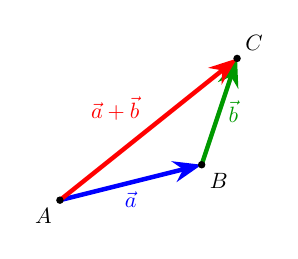
\begin{tikzpicture}[>=Stealth, thick, scale=0.9, every node/.style={scale=0.8}]
                \coordinate (A) at (0,0);
                \coordinate (B) at (2,0.5);
                \coordinate (C) at (2.5,2);

                \draw[->, blue, ultra thick] (A) -- (B) node[midway, below] {$\vec{a}$};
                \draw[->, green!60!black, ultra thick] (B) -- (C) node[midway, right] {$\vec{b}$};
                \draw[->, red, ultra thick] (A) -- (C) node[midway, above left] {$\vec{a} + \vec{b}$};

                \fill (A) circle (1.5pt) node[below left] {$A$};
                \fill (B) circle (1.5pt) node[below right] {$B$};
                \fill (C) circle (1.5pt) node[above right] {$C$};
            \end{tikzpicture}
        \end{column}
    \end{columns}

    % \vspace{0.2cm} % Khoảng cách giữa 2 phần

    % --- PHẦN 2: QUY TẮC HÌNH BÌNH HÀNH ---
    \begin{columns}[c]
        \begin{column}{0.5\textwidth}
            \begin{block}{Quy tắc Hình bình hành (Parallelogram Law)}
                \footnotesize
                Nếu $\vec{a}, \vec{b}$ chung điểm đầu $O$:
                \[ \vec{a} + \vec{b} = \vec{OA} + \vec{OB} = \vec{OC} \]
                (với $OC$ là đường chéo hình bình hành $OACB$)
            \end{block}
        \end{column}
        
        \begin{column}{0.45\textwidth}
            \centering
            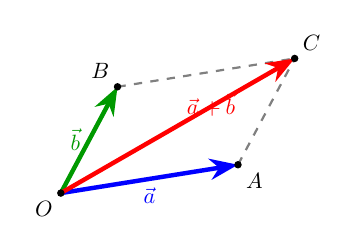
\begin{tikzpicture}[>=Stealth, thick, scale=0.9, every node/.style={scale=0.8}]
                \coordinate (O) at (0,0);
                \coordinate (A) at (2.5,0.4);
                \coordinate (B) at (0.8,1.5);
                \coordinate (C) at (3.3,1.9); 

                \draw[dashed, gray] (A) -- (C);
                \draw[dashed, gray] (B) -- (C);
                \draw[->, blue, ultra thick] (O) -- (A) node[midway, below] {$\vec{a}$};
                \draw[->, green!60!black, ultra thick] (O) -- (B) node[midway, left] {$\vec{b}$};
                \draw[->, red, ultra thick] (O) -- (C) node[midway, above right] {$\vec{a} + \vec{b}$};

                \fill (O) circle (1.5pt) node[below left] {$O$};
                \fill (A) circle (1.5pt) node[below right] {$A$};
                \fill (B) circle (1.5pt) node[above left] {$B$};
                \fill (C) circle (1.5pt) node[above right] {$C$};
            \end{tikzpicture}
        \end{column}
    \end{columns}

    \vspace{0.1cm}
    \centering
    \footnotesize \textbf{Ghi chú:} Cả hai quy tắc đều cho cùng một kết quả vector tổng.
\end{frame}



\subsection{Phép trừ hai vector (Vector Subtraction)}

\begin{frame}[fragile]
    \frametitle{\thesection. \insertsection}
    \framesubtitle{\thesection.\thesubsection. \insertsubsection}

    \vspace{-0.3cm}

    % --- PHẦN 1: QUY TẮC HIỆU CHUNG GỐC ---
    \begin{columns}[c]
        \begin{column}{0.5\textwidth}
            \begin{block}{Hiệu chung gốc (Subtraction Rule)}
                \footnotesize
                Cho $\vec{a} = \vec{AB}, \vec{b} = \vec{AC}$ (chung điểm đầu $A$). Hiệu của chúng là:
                \[ \vec{a} - \vec{b} = \vec{AB} - \vec{AC} = \vec{CB} \]
                \textbf{Ghi nhớ:} Vector hiệu hướng từ ngọn của số trừ ($C$) đến ngọn của số bị trừ ($B$).
            \end{block}
        \end{column}
        
        \begin{column}{0.45\textwidth}
            \centering
            \vspace{0.3cm}
            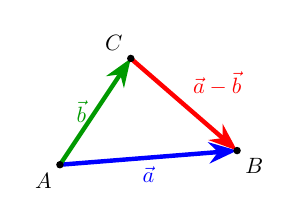
\begin{tikzpicture}[>=Stealth, thick, scale=0.9, every node/.style={scale=0.8}]
                \coordinate (A) at (0,0);
                \coordinate (B) at (2.5,0.2);
                \coordinate (C) at (1,1.5);

                \draw[->, blue, ultra thick] (A) -- (B) node[midway, below] {$\vec{a}$};
                \draw[->, green!60!black, ultra thick] (A) -- (C) node[midway, left] {$\vec{b}$};
                \draw[->, red, ultra thick] (C) -- (B) node[midway, above right] {$\vec{a} - \vec{b}$};

                \fill (A) circle (1.5pt) node[below left] {$A$};
                \fill (B) circle (1.5pt) node[below right] {$B$};
                \fill (C) circle (1.5pt) node[above left] {$C$};
            \end{tikzpicture}
        \end{column}
    \end{columns}

    % --- PHẦN 2: CỘNG VỚI VECTOR ĐỐI ---
    \begin{columns}[c]
    \begin{column}{0.5\textwidth}
        \begin{block}{Cộng với vector đối (Negative Vector)}
            \footnotesize
            Phép trừ thực chất là cộng với vector đối $-\vec{b}$ của $\vec{b}$:
            \[ \vec{a} - \vec{b} = \vec{OA} - \vec{OB} = \vec{OA} + \vec{BO} = \vec{BA} \]
            (Trong đó $\vec{BO} = -\vec{OB} = -\vec{b}$ là vector đối của $\vec{b}$)
        \end{block}
    \end{column}
    
    \begin{column}{0.45\textwidth}
        \centering
        \begin{tikzpicture}[>=Stealth, thick, scale=0.9, every node/.style={scale=0.8}]
            \coordinate (O) at (0,0);
            \coordinate (A) at (2.5,0.2);
            \coordinate (B) at (1,1.5);
            \coordinate (BO) at (-1,-1.5); % vector BO (đối của OB)

            % Vecto a = OA (màu xanh dương)
            \draw[->, blue, ultra thick] (O) -- (A) node[midway, below] {$\vec{a}$};
            
            % Vecto b = OB ban đầu (vẽ mờ để thấy sự đối)
            \draw[->, gray, thin] (O) -- (B) node[midway, right] {$\vec{b}$};
            
            % Vecto đối -b = BO (xanh lá)
            \draw[->, green!60!black, ultra thick] (O) -- (BO) node[midway, left] {$-\vec{b}$};
            
            % Tổng a + (-b) = a - b (quy tắc hình bình hành)
            \coordinate (A_plus_BO) at ($(A) + (BO)$);
            \draw[dashed, gray] (A) -- (A_plus_BO);
            \draw[dashed, gray] (BO) -- (A_plus_BO);
            \draw[->, red, ultra thick] (O) -- (A_plus_BO) node[midway, below right] {$\vec{a} - \vec{b}$};

            \fill (O) circle (1.5pt) node[below left] {$O$};
            \fill (A) circle (1.5pt) node[below right] {$A$};
            \fill (B) circle (1.5pt) node[above right] {$B$};
        \end{tikzpicture}
    \end{column}
\end{columns}

\vspace{0.1cm}
\centering
\footnotesize \textbf{Ghi chú:} Phép trừ đưa về phép cộng giúp vận dụng được quy tắc hình bình hành và tam giác.

\end{frame}



\subsection{Phép nhân vô hướng (Scalar Multiplication)}

\begin{frame}[fragile]
    \frametitle{\thesection. \insertsection}
    \framesubtitle{\thesection.\thesubsection. Nhân vector với một số (Scalar Multiplication)}

    \begin{columns}[T, onlytextwidth]
        \begin{column}{0.5\textwidth}
            \begin{block}{Định nghĩa}
                \footnotesize
                Cho số thực $k \neq 0$ và vector $\vec{a} \neq \vec{0}$. Tích $k\vec{a}$ là một vector:
                \begin{itemize}
                    \item Cùng hướng với $\vec{a}$ nếu $k > 0$.
                    \item Ngược hướng với $\vec{a}$ nếu $k < 0$.
                    \item Độ dài: $|k\vec{a}| = |k| \cdot |\vec{a}|$.
                \end{itemize}
            \end{block}

            \begin{exampleblock}{Ví dụ}
                \footnotesize
                $\vec{a} = (2, 1)$:
                \begin{itemize}
                    \item $2\vec{a} = (4, 2)$ (cùng hướng, dài gấp đôi)
                    \item $-1.5\vec{a} = (-3, -1.5)$ (ngược hướng)
                \end{itemize}
            \end{exampleblock}
        \end{column}
        
        \begin{column}{0.45\textwidth}
            \centering
            \begin{tikzpicture}[>=Stealth, thick, scale=0.9, every node/.style={scale=0.8}]
                \draw[->, gray!50, thin] (-3.5,0) -- (4,0) node[right] {$x$};
                \draw[->, gray!50, thin] (0,-2.5) -- (0,2.5) node[above] {$y$};
                
                \coordinate (O) at (0,0);
                \coordinate (A) at (2,1);
                \coordinate (A2) at (4,2);
                \coordinate (A_neg) at (-3,-1.5);
                
                \draw[->, blue, ultra thick] (O) -- (A) node[midway, above left] {$\vec{a}$};
                \draw[->, red, ultra thick] (O) -- (A2) node[midway, above left] {$2\vec{a}$};
                \draw[->, green!60!black, ultra thick] (O) -- (A_neg) node[midway, below right] {$-1.5\vec{a}$};
                
                \fill (O) circle (1.5pt) node[below left] {$O$};
            \end{tikzpicture}
        \end{column}
    \end{columns}

    \vspace{0.2cm}
    \begin{center}
        \footnotesize \textbf{Ghi chú:} $k=0$ hoặc $\vec{a}=\vec{0}$ thì $k\vec{a}=\vec{0}$.
    \end{center}
\end{frame}


\begin{frame}[fragile]
    \frametitle{\thesection. \insertsection}
    \framesubtitle{\thesection.\thesubsection. Tích vô hướng của hai vector (Dot Product)}

    \begin{columns}[T, onlytextwidth]
        \begin{column}{0.52\textwidth}
            \begin{block}{Định nghĩa hình học (Geometric Definition)}
                \footnotesize
                Tích vô hướng của $\vec{a}$ và $\vec{b}$ là một số thực:
                \[
                    \vec{a} \cdot \vec{b} = |\vec{a}| \cdot |\vec{b}| \cdot \cos\theta
                \]
                với $\theta = (\vec{a}, \vec{b})$ là góc giữa hai vector.
            \end{block}
            
            \vspace{0.3cm}
            
            \begin{block}{Định nghĩa tọa độ (Coordinate Definition)}
                \footnotesize
                Trong mặt phẳng $Oxy$, cho $\vec{a} = (x_1, y_1)$, $\vec{b} = (x_2, y_2)$:
                \[
                    \vec{a} \cdot \vec{b} = x_1 x_2 + y_1 y_2
                \]
            \end{block}
        \end{column}
        
        \begin{column}{0.44\textwidth}
            \centering
            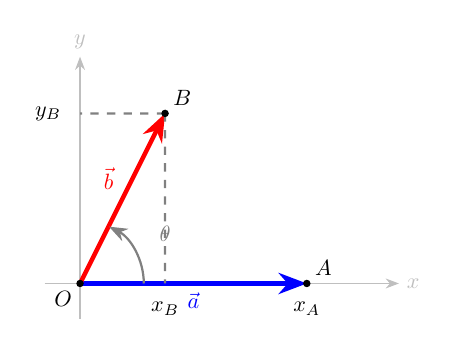
\begin{tikzpicture}[>=Stealth, thick, scale=0.9, every node/.style={scale=0.8}]
                % Trục tọa độ
                \draw[->, gray!50, thin] (-0.5,0) -- (4.5,0) node[right] {$x$};
                \draw[->, gray!50, thin] (0,-0.5) -- (0,3.2) node[above] {$y$};
                
                % Điểm O, A, B
                \coordinate (O) at (0,0);
                \coordinate (A) at (3.2,0);
                \coordinate (B) at (1.2,2.4);
                
                % Vẽ vector a và b
                \draw[->, blue, ultra thick] (O) -- (A) node[midway, below] {$\vec{a}$};
                \draw[->, red, ultra thick] (O) -- (B) node[midway, above left] {$\vec{b}$};
                
                % Góc theta
                \draw[->, gray, thick] (0.9,0) arc[start angle=0, end angle=63, radius=0.9];
                \node[gray] at (1.2,0.7) {$\theta$};
                
                % Đường gióng tọa độ của A
                \draw[dashed, gray] (A) -- (3.2,0);
                
                % Đường gióng tọa độ của B
                \draw[dashed, gray] (B) -- (1.2,0);
                \draw[dashed, gray] (B) -- (0,2.4);
                
                % Ký hiệu x_A, y_A, x_B, y_B
                \node[below] at (3.2, -0.15) {$x_A$};
                \node[below] at (1.2, -0.15) {$x_B$};
                \node[left] at (-0.15, 2.4) {$y_B$};
                
                % Điểm A, B (dịch ra xa hơn để không trùng)
                \fill (O) circle (1.5pt) node[below left] {$O$};
                \fill (A) circle (1.5pt) node[above right] {$A$};
                \fill (B) circle (1.5pt) node[above right] {$B$};
            \end{tikzpicture}
            
            \vspace{0.2cm}
            \begin{center}
                \footnotesize
                $\vec{a} \cdot \vec{b} = OA \cdot OB \cdot \cos\theta = x_A x_B + y_A y_B$
            \end{center}
        \end{column}
    \end{columns}

    \vspace{0.2cm}
    \begin{center}
        \footnotesize \textbf{Ghi chú:} Tích vô hướng là số (scalar), khác với tích vector.
    \end{center}
\end{frame}



\subsection{Góc giữa hai vector (Angle between two vectors)}

\begin{frame}[fragile]
    \frametitle{\thesection. \insertsection}
    \framesubtitle{\thesection.\thesubsection. Góc giữa hai vector (Angle between two vectors)}

    \begin{columns}[T, onlytextwidth]
        \begin{column}{0.5\textwidth}
            \footnotesize
            \textbf{Từ định nghĩa tích vô hướng:}
            \[
                \vec{a} \cdot \vec{b} = |\vec{a}| \cdot |\vec{b}| \cdot \cos\theta
            \]
            với $\theta = (\vec{a}, \vec{b})$ là góc giữa hai vector.
            
            \vspace{0.2cm}
            
            \begin{block}{Côsin của góc (Cosine formula)}
                \centering
                \[
                    \cos\theta = \frac{\vec{a} \cdot \vec{b}}{|\vec{a}| \cdot |\vec{b}|}
                \]
                \vspace{0.1cm}
                \textbf{Dạng tọa độ:}
                \[
                    \cos\theta = \frac{x_1 x_2 + y_1 y_2}{\sqrt{x_1^2 + y_1^2} \cdot \sqrt{x_2^2 + y_2^2}}
                \]
            \end{block}
        \end{column}
        
        \begin{column}{0.46\textwidth}
            \centering
            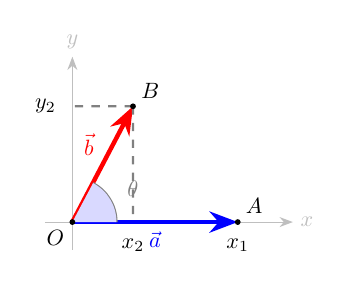
\begin{tikzpicture}[>=Stealth, thick, scale=0.7, every node/.style={scale=0.8}]
                % Trục tọa độ
                \draw[->, gray!50, thin] (-0.5,0) -- (4,0) node[right] {$x$};
                \draw[->, gray!50, thin] (0,-0.5) -- (0,3) node[above] {$y$};
                
                % Điểm O, A, B
                \coordinate (O) at (0,0);
                \coordinate (A) at (3,0);
                \coordinate (B) at (1.1,2.1);
                
                % Vẽ vector a và b
                \draw[->, blue, ultra thick] (O) -- (A) node[midway, below] {$\vec{a}$};
                \draw[->, red, ultra thick] (O) -- (B) node[midway, above left] {$\vec{b}$};
                
                % Góc theta
                \draw[gray, thick] (0.8,0) arc[start angle=0, end angle=62, radius=0.8];
                \node[gray] at (1.1,0.6) {$\theta$};
                
                % Tô vùng góc
                \fill[blue!15] (0,0) -- (0.8,0) arc[start angle=0, end angle=62, radius=0.8] -- cycle;
                
                % Đường gióng tọa độ
                \draw[dashed, gray] (A) -- (3,0);
                \draw[dashed, gray] (B) -- (1.1,0);
                \draw[dashed, gray] (B) -- (0,2.1);
                
                % Ký hiệu tọa độ
                \node[below] at (3, -0.15) {$x_1$};
                \node[below] at (1.1, -0.15) {$x_2$};
                \node[left] at (-0.15, 2.1) {$y_2$};
                
                % Điểm
                \fill (O) circle (1.5pt) node[below left] {$O$};
                \fill (A) circle (1.5pt) node[above right] {$A$};
                \fill (B) circle (1.5pt) node[above right] {$B$};
            \end{tikzpicture}
            
            \vspace{0.3cm}
            
            \begin{block}{Tính chất}
                \centering
                \begin{tabular}{ll}
                    $\vec{a} \cdot \vec{b} > 0$ & $\Rightarrow \theta < 90^\circ$ (góc nhọn)\\
                    $\vec{a} \cdot \vec{b} = 0$ & $\Rightarrow \theta = 90^\circ$ (vuông góc)\\
                    $\vec{a} \cdot \vec{b} < 0$ & $\Rightarrow \theta > 90^\circ$ (góc tù)
                \end{tabular}
            \end{block}
        \end{column}
    \end{columns}

\end{frame}


\section{Tổng kết}
\subsection{Các công thức quan trọng}

\begin{frame}[fragile]
    \frametitle{\thesection. \insertsection}
    \framesubtitle{\thesection.\thesubsection. Các công thức cần nhớ}

    \begin{block}{Tổng hợp công thức vector}
        \vspace{0.2cm} % Thêm khoảng cách giữa tiêu đề và nội dung
        \begin{columns}[T, onlytextwidth]
            \begin{column}{0.5\textwidth}
                \textbf{1. Cộng vector:} $\vec{AB}+\vec{BC}=\vec{AC}$ (tam giác); $\vec{OA}+\vec{OB}=\vec{OC}$ (hbh) \\
                \vspace{0.15cm}
                \textbf{2. Trừ vector:} $\vec{AB}-\vec{AC}=\vec{CB}$; $\vec{a}-\vec{b}=\vec{a}+(-\vec{b})$ \\
                \vspace{0.15cm}
                \textbf{3. Nhân với số:} $k\vec{a}=(kx,ky)$, $|k\vec{a}|=|k|\cdot|\vec{a}|$ ($k>0$ cùng hướng, $k<0$ ngược) \\
                \vspace{0.15cm}
                \textbf{4. Tọa độ:} $\vec{AB}=(x_B-x_A,\;y_B-y_A)$; $|\vec{a}|=\sqrt{x^2+y^2}$
            \end{column}

            \hspace{0.5cm}

            \begin{column}{0.5\textwidth}
                \textbf{5. Tích vô hướng:} $\vec{a}\cdot\vec{b}=|\vec{a}||\vec{b}|\cos\theta=x_1x_2+y_1y_2$ \\
                \vspace{0.15cm}
                \textbf{6. Côsin góc:} $\cos\theta=\dfrac{\vec{a}\cdot\vec{b}}{|\vec{a}||\vec{b}|}=\dfrac{x_1x_2+y_1y_2}{\sqrt{x_1^2+y_1^2}\sqrt{x_2^2+y_2^2}}$ \\
                \vspace{0.15cm}
                \textbf{7. Vuông góc:} $\vec{a}\perp\vec{b}\iff\vec{a}\cdot\vec{b}=0\iff x_1x_2+y_1y_2=0$
            \end{column}
        \end{columns}
        \vspace{0.1cm}
    \end{block}

    \begin{center}
        \footnotesize $\vec{a}=(x_1,y_1)$, $\vec{b}=(x_2,y_2)$
    \end{center}
\end{frame}

\end{document}